% Se configura el tipo de documento
\documentclass[a4paper]{scrartcl}

%THIS IS TO MAKE THE DOCUMENT PRETTIER
\usepackage[utf8]{inputenc}
\usepackage[spanish, es-tabla, es-nodecimaldot]{babel}

\usepackage[T1]{fontenc}
\usepackage{lmodern} %AGREGO1
\usepackage{fourier}			% English language/hyphenation

\usepackage{color}
\usepackage[protrusion=true,expansion=true]{microtype}
\usepackage{amsmath}
\usepackage{amsfonts,amsthm} % Math packages
\usepackage[pdftex]{graphicx}
\usepackage{url}
\usepackage{import}
\usepackage{multicol}

\usepackage[margin=2cm]{geometry}

% %%% Custom sectioning
\usepackage{sectsty}
\allsectionsfont{\normalfont \scshape} 

%%% Custom headers/footers (fancyhdr package)
\usepackage{fancyhdr}
\pagestyle{fancyplain}

\fancyhead{}											% No page header
\fancyfoot[L]{}											% Empty
\fancyfoot[C]{}											% Empty
\fancyfoot[R]{\thepage}									% Pagenumbering
\renewcommand{\headrulewidth}{0pt}			% Remove header underlines
\renewcommand{\footrulewidth}{0pt}				% Remove footer underlines
\setlength{\headheight}{13.6pt}

\usepackage{float}

%%% Equation and float numbering
\numberwithin{equation}{section}		% Equationnumbering: section.eq#
\numberwithin{figure}{section}			% Figurenumbering: section.fig#
\numberwithin{table}{section}				% Tablenumbering: section.tab#

%%% Maketitle metadata
\newcommand{\horrule}[1]{\rule{\linewidth}{#1}} 	% Horizontal rule
%FINISHED MAKING PRETTIER DOCUMENT



% --------------ADDED BY FACUNDO FARALL--------------

%MATHEMATICS PACKAGES
\usepackage{amsmath,amsfonts,amsthm}
%FINISHED MATHEMATICS



%THIS IS SO THAT REFERENCES CAN BE CLICKED
\usepackage{hyperref}
\hypersetup{
    colorlinks=true,
    linkcolor=blue,
    filecolor=magenta,      
    urlcolor=blue,
    citecolor=blue,    
}
%FINISHED CLICKABLE REFERENCES



%THIS IS TO CHANGE MARGINES FOR SITUATIONS LIKE LONG EQUATIONS
\usepackage[strict]{changepage}
%ENDS CHANGER OF MARGINS



%THIS IS TO USE SMALLER FONT SIZE
\usepackage[11pt]{moresize}
%FINISHED FONT SIZE CHANGER



%THE FOLLOWING ARE CONFIGURATIONS FOR TODONOTES
\usepackage{todonotes,varwidth}
\makeatletter
\tikzstyle{diaanotestyle} = [
    draw=\@todonotes@currentbordercolor,
    fill=\@todonotes@currentbackgroundcolor,
    line width=0.5pt,
    inner sep = 0.8 ex,
    rounded corners=4pt,align=left,
   ]

\renewcommand{\@todonotes@drawInlineNote}{%
        {\begin{tikzpicture}[remember picture,baseline={(0,0)}]%
            \draw node[diaanotestyle,font=\@todonotes@sizecommand,anchor=base west]{%
               \begin{varwidth}[t]{10cm}
                \if@todonotes@authorgiven%
                    {\@todonotes@sizecommand \@todonotes@author:\,\@todonotes@text}%
                \else%
                    {\@todonotes@sizecommand \@todonotes@text}%
                \fi
                \end{varwidth}};%
            \end{tikzpicture}}%
       }%
\makeatother
%HERE ENDS THE CONFIGURATIONS FOR TODONOTES

% --------------ENDS ADDED BY FACUNDO FARALL--------------

\begin{document}

\title{
	\usefont{OT1}{bch}{b}{n}
	\normalfont \normalsize \textsc{Instituto Tecnol\'ogico de Buenos Aires} \\ [25pt]
	\horrule{2pt} \\[0.4cm]
	\huge Trabajo Pr\'actico Nº 1\\ Configuraci\'on Darlington \\
	\horrule{2pt} \\[0cm]
\author{\\Grupo 2:\\\\Francois, Mat\'ias\\Maselli, Carlos\\ M\"uller, Malena\\ Trozzo, Nicol\'as\\ \\ \\ \\
Profesores: \\\\ Alcocer, Fernando\\ Oreglia, Eduardo Victor \\Gardella, Pablo Jes\'us\\ \\ } 
\text{Electr\'onica I - 2019}
}
\date{\today} 
\pagenumbering{arabic}

\maketitle
\newpage

% Crear indice del informe
\tableofcontents

% Incluyendo los ejercicios realizados
\newpage
\section{Introducci\'on}

La configuraci\'on ''Darlington'', tambi\'en conocida como ''par Darlington'', consiste en dos transistores conectados como se observa en la figura \ref{darlington_ideal}, en colector común, con el fin de obtener una mayor ganancia de corriente respecto a la obtenida al emplear un \'unico transistor en la misma configuración. Se analiza el comportamiento del circuito para comprender la utilidad del par Darlington, muy utilizado como buffer, o seguidor de tensión. Se comienza por un an\'alisis te\'orico del circuito para luego implementarlo utilizando utilizando los transistores BC337-40\footnote{Hoja de datos del transistor BC337-40: https://pdf1.alldatasheet.com/datasheet-pdf/view/156199/ONSEMI/BC337-40.html}.

\begin{figure}[H]
	\centering
		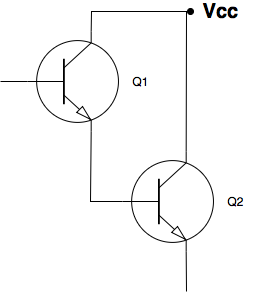
\includegraphics[scale=0.4]{./Imagenes/darlington_ideal.png} 
	\caption{Configuraci\'on Darlington.}
	\label{darlington_ideal}
\end{figure}

\newpage

\section{Análisis teórico del circuito}



	\subsection{Polarizaci\'on}
		En la Figura \ref{polarizacion} se muestra el modelo del circuito considerando que los capacitores representan circuitos abiertos, ya que en este caso se trabaja con tensión $V_{cc}$ continua. El mismo se esquematiza con el equivalente de Thevenin entre el nodo de base y masa.\\
		\begin{figure}[H]
			\centering
			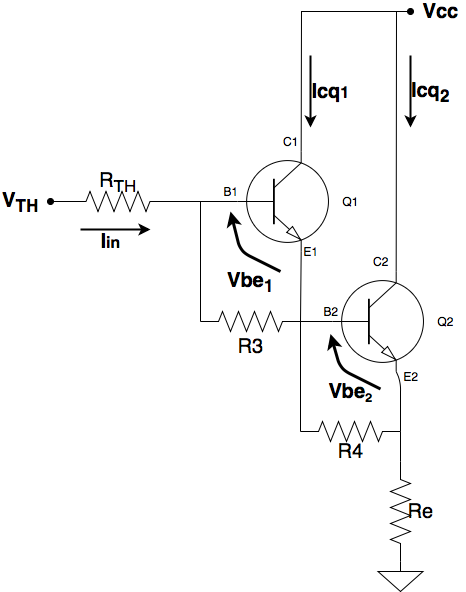
\includegraphics[scale=0.4]{./Imagenes/polarizacion.png} \\
			\caption{Circuito equivalente para el an\'alisis de polarizaci\'on.}
			\label{polarizacion}
		\end{figure}

Los valores utilizados para los cálculos son los de los componentes que utilizados en la implementación del circuito, que fueron elegidos en base a las simulaciones realizadas, con el fin de lograr un resultado óptimo. De esta forma, los valores de los componentes utilizados se listan en la Tabla \ref{tabla_valores}. Los transistores utilizados son BC337-40.

\begin{table}[H]
\centering
\begin{tabular}{ll}
\hline
\multicolumn{2}{l}{\begin{tabular}[c]{@{}l@{}}Parámetros\\   del circuito\end{tabular}} \\ \hline
$V_{cc}$                                     & $15V$                         \\
$R_1$                                         & $100 k\Omega$                           \\
$R_2$                                         & $330k\Omega$                              \\
$R_s$                                         & $10k\Omega$                             \\
$R_3$                                         & $10k\Omega$                          \\
$R_E$                                         & $4,7k\Omega$                               \\
$R_L$                                         & $1k\Omega$                           
\end{tabular}
\caption{Valores de los componentes utilizados}
\label{tabla_valores}  
\end{table}

El equivalente de Thevenin entre la base del primer transistor y masa se obtiene mediante:\\

	\begin{equation}
		\begin{cases}
		&V_{TH} = \frac{R_2}{R_1 + R_2} V_{CC}\\ \\
		&R_{TH} = R_1 // R_2 
		\end{cases}
		\label{Thevenin}
	\end{equation}

Recorriendo la malla de entrada se tiene que:
\begin{equation}
		V_{th}-I_{B1}R_{th}-V_{BEon_{1}}-V_{BEon_{2}}-R_{e}(I_{E_{2}}+I_{R_{3}})=0 
\end{equation}
Del nodo que conecta el emisor del primer transistor con la base del segundo, se relacionan las corrientes de los transistores:
\begin{equation}
		I_{B_{2}} = I_{E_{1}} - \frac{V_{BEon_{2}}}{R_{3}}
\end{equation}
Por último, de las ecuaciones de cada transistor, despreciando el efecto de las $I_{CB0}$ dado que se trabaja a temperatura ambiente, se verifica:

	\begin{equation}
		\begin{cases}
		Q_{1}) \, \, I_{E_{1}} = I_{B_{1}}(\beta_{1}+1)\\ \\
		Q_{2}) I_{E_{2}}=I_{B_{2}}(\beta_{2}+1)
		\end{cases}
	\end{equation}

Resolviendo dichas ecuaciones se llega a las siguientes expresiones para las corrientes de colector de ambos transistores:

	\begin{equation}
		\begin{cases}
		I_{cq_{1}}=\frac{V_{th}-V_{BEon_{1}}-V_{BEon_{2}}\left(1-\frac{R_{e}\beta_{2}}{R_{3}}\right)}{\frac{R_{th}}{\beta_{1}}+R_{e}\beta_{2}}\\ \\
		I_{cq_{2}}=V_{th}\frac{1}{\frac{R_{th}}{\beta_{1}\beta_{2}}+R_{e}\frac{\beta_{2}+1}{\beta_{2}}}-V_{BEon_{1}}\frac{1}{\frac{R_{th}}{\beta_{2}}+R_{e}\beta_{1}}-V_{BEon_{2}}\left(\frac{\beta_{2}}{R_{3}}+\frac{\left(1-\frac{R_{e}\beta_{2}}{R_{3}}\right)\cdot(\beta_{1}+1)}{\frac{R_{th}}{\beta_{2}}+R_{e}\beta_{1}} \right)
		\end{cases}
	\end{equation}

Por último, se puede verificar que ambos transistores queden correctamente polarizados mediante:

	\begin{equation}
		\begin{cases}
		V_{CEQ_{1}}=V_{CC}-V_{BEon_{2}}\left(1+\frac{R_{e}}{R_{3}}\right)-R_{e}I_{CQ_{2}}\\ \\
		V_{CEQ_{2}}=V_{CC}-V_{BEon_{2}}\frac{R_{e}}{R_{3}}-R_{e}I_{CQ_{2}}
		\end{cases}
	\end{equation}
	

Para los cálculos se utiliza $V_{BEon}=0.7(V)$ para ambos transistores. Con respecto a los $H_{FE}$, éstos dependen de las $I_{CQ}$ según la \href{https://pdf1.alldatasheet.com/datasheet-pdf/view/171970/ONSEMI/BC337-40.html}{hoja de datos del fabricante}, con lo que son distintos para cada transistor. Tomando inicialmente el $H_{FE}$ mínimo de la hoja de datos, e iterando para los valores de $I_{CQ}$ obtenidos, se llega a que:
	\begin{equation*}
		\begin{cases}
		 H_{FE1} = 47\\
		 H_{FE2} = 90
		\end{cases}
	\end{equation*}
Reemplazando además por los valores de los componentes utilizados, se hallan los valores de $I_{cq_{1}}$, $I_{cq_{2}}$, $V_{CEQ_{1}}$ y $V_{CEQ_{2}}$, detallados en la Tabla \ref{tabla_valores_polarizacion}.

\begin{table}[H]
	\centering
\begin{tabular}{ll}
\multicolumn{2}{l}{Polarización} \\ \hline
$I_{CQ1}$          & $93,54\mu A$       \\
$I_{CQ2}$        & $2,12mA$        \\
$V_{CEQ1}$         & $4,01V$       \\
$V_{CEQ2}$         & $4,71V$      
\end{tabular}
\caption{Valores hallados para las componentes de polarizacion.}
\label{tabla_valores_polarizacion}  
\end{table}


	\subsection{Modelo incremental}
	
	Los estimadores para los parámetros del modelo incremental de cada transistor se detallan a continuación.

		\begin{equation}
			\begin{cases}
			\widehat{r_{e}}=\frac{V_{T}}{I_{CQ}}\\
			{\widehat{h}_{ie}}=(\beta+1)R_{e}\\	
			{\widehat{g}_m}=\frac{1}{r_{e}}\\
			{\widehat{h}_{fe}}= \beta_{DC}\\
			\widehat{\frac{1}{h_{oe}}}= \infty
			\end{cases}
			\label{mod_inc_ecs}
		\end{equation}
		
	Se utiliza la ganancia de continua como estimador dado que las hojas de datos no especifican un valor para $h_{fe}$. Utilizando los valores de las corrientes de polarización y $h_{fe}$ de cada transistor, se obtienen los siguientes valores:
	
	\todo{COMPLETAR TABLA de estimadores}
	\begin{table}[h!]
		\centering
		\begin{tabular}{c c c}%
			\bfseries Estimadores & Q1 & Q2 \\ \hline
			$\widehat{g}_m$ &  & \\
			$\widehat{h}_{ie}$ &  & \\
			$\widehat{r}_{e}$&  & \\
			\hline
		\end{tabular}
		\caption{Estimadores correspondientes al modelo incremental, para los transistores Q1 y Q2.}
		\label{avolf}
	\end{table}
	
	\subsection{Circuito incremental}
	
	En la Figura \ref{circ_incremental} se muestra el circuito incremental. Las resistencias de salida de cada transistor se desprecian en los cálculos ya que hacerlo no introduce un error considerable y simplifica las operaciones.
		\begin{figure}[H]
			\centering
			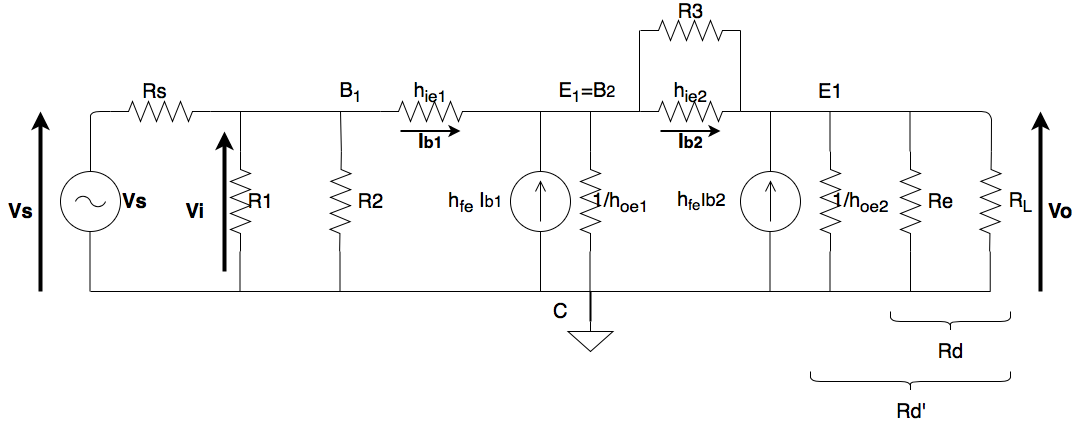
\includegraphics[scale=0.4]{./Imagenes/circ_incremental.png} \\
			\caption{Circuito equivalente para el an\'alisis del circuito incremental.}
			\label{circ_incremental}
		\end{figure}

En la Tabla \ref{tabla_valores_incremental} se muestran los valores utilizados y calculados en esta sección, que se utilizan para calcular las ganancias e impedancias del circuito.

\begin{table}[H]
\centering
\begin{tabular}{ll}
\multicolumn{2}{l}{Modelo incremental} \\ \hline
$V_T$              & 26mV             \\
$h_{fe1}$           & 47            \\
$h_{fe2}$           & 90            \\
$h_{ie1}$            & 13,34$k\Omega$            \\
$h_{ie2}$           & 1,12$k\Omega$             \\
\end{tabular}
\label{tabla_valores_incremental} 
\end{table}

Para poder resolver el circuito fácilmente, se agrupa en paralelo la resistencia $R_3$ con $hie2$. Para poder hacerlo, se debe también adaptar la fuente de corriente del segundo transistor por la que circula por el paralelo de las resistencias de la siguiente forma. Además, se agrupan en paralelo $R_e$ y $R_L$. Para éstas consideraciones se calculan los siguientes parámetros:

	\begin{equation}
		\begin{cases}
		h{fe2}^{*}=h_{fe2}\frac{R_{3}}{R_{3}+h_{ie2}} \\
		h_{ie2}^{*}=h_{ie2}//R_{3} \\
		R_{d}=R_{e}//R_{2}
		\end{cases}
		\label{mod_inc_ecs}
	\end{equation}

Reemplazando por los valores correspondientes se obtienen los siguientes valores:

\begin{table}[H]
\centering
\begin{tabular}{ll}
\multicolumn{2}{l}{Simplificaciones} \\ \hline
$h_{fe2}*$          & 80,96           \\
$R_d$             & 824,56$\Omega$          \\
$h_{ie2}*$          & 1,00$k\Omega$          
\end{tabular}
\end{table}

A partir del circuito y de los cálculos anteriores, se puede ver que las expresiones para las impedancias que se ven a la entrada del primer transistor, del amplificador y del sistema se ven representadas por las ecuaciones que se muestran a continuación, utilizando pasaje a nivel de corriente. 

	\begin{equation}
		\begin{cases}	
		R_{i}=hie_{1}+(hfe_{1}+1)hie_{2}^{*}+(hfe_{2}^{*}+1)(hfe_{1}+1)R_{d} \\
		R_{ia}=R_{i} // R_{th} \\
		R_{is}=R_{s}+R_{ia}
		\end{cases}
		\label{mod_inc_ecs}
	\end{equation}

De donde reemplanzando por los valores ya calculados se obtienen las impedancias de entrada:

\begin{table}[H]
\centering
\begin{tabular}{ll}
\multicolumn{2}{l}{\begin{tabular}[c]{@{}l@{}}Impedancias\\   de entrada\end{tabular}} \\ \hline
$R_i$                                      & 3,31$M\Omega$                                     \\
$R_{ia}$                                     & 75,00$k\Omega$                                    \\
$R_{is}$                                    & 85,00$k\Omega$                                   
\end{tabular}
\end{table}

Para el cálculo de la ganancia de tensión del sistema primero se calcula:

	\begin{equation}
		\begin{cases}	
		\frac{V_{o}}{ib_{2}^{*}}=R_{d}(hfe_{2}^{*}+1) \\
		\frac{V_{i}}{V_{s}}=\frac{R_{ia}}{R_{ia}+R_{s}}
		\end{cases}
		\label{mod_inc_ecs}
	\end{equation}

Así la ecuación de la ganancia en tensión del sistema se puede expresar de la siguiente forma. \\

	\begin{equation}	
		\Delta _{vs}=\frac{V_{o}}{V_{s}}=\frac{V_{o}}{ib_{2}^{*}}\cdot\frac{ib_{2}^{*}}{ib_{1}}\cdot\frac{ib_{1}}{V_{i}}\cdot\frac{V_{i}}{V_{s}}=R_{d}(hfe_{2}^{*}+1)(hfe_{1}+1)\frac{1}{R_{i}}\frac{Ria}{Ria+Rs}
		\label{mod_inc_avs}
	\end{equation}

Finalmente, se llega a los valores de las ganancias de tensión del amplificador y del sistema:

\begin{table}[H]
\centering
\begin{tabular}{ll}
\multicolumn{2}{l}{\begin{tabular}[c]{@{}l@{}}Ganancias\\   de tension\end{tabular}} \\ \hline
$Av$                                       & 0,981                                     \\
$Avs$                                      & 0,866                                    
\end{tabular}
\end{table}

Al ser la configuración colector común se esperaba una ganancia de tensión menor a 1. De éste resultado se puede observar una ventaja de la configuración Darlington con respecto al colector común con un solo transistor, ya que éste último no puede llegar valores de ganancia de tensión superiores al 80\%.\\
Para el cálculo de la ganancia de corriente se utiliza:

	\begin{align*}
		\Delta _{i} &= \frac{I_{Rd}}{ib_{1}}=(hfe_{2}^{*}+1)(hfe_{1}+1) \\
%
	\Delta_{is} &= \frac{I_{Rd}}{I_{Rs}}\cdot\frac{I_{b_{1}}}{I_{Rs}}=\frac{R_{th}}{R_{th}+R_{i}}\Delta_{i} \\
%
		\Delta_{is}^{\, \, \,'} &= \frac{I_{Rl}}{I_{Rs}}=\frac{I_{Rl}}{I_{Rd}}\cdot\frac{I_{Rd}}{I_{Rs}}=\frac{R_{e}}{R_{e}	+R_{2}}\Delta_{is}
%
		\label{mod_inc_ais}
	\end{align*}


Donde $\Delta_{i}$ es la ganancia de corriente, $\Delta_{is}$ es la ganancia de corriente del sistema y $\Delta_{is}^{\, \, \,'}$ es la ganancia de corriente del sistema sobre la carga. En $\Delta_{i}$ se puede apreciar la gran ganancia de corriente que tiene esta configuración, ya que se multiplican las ganancias de cada transistor. Los valores de las mismas se muestran en la siguiente tabla:

\begin{table}[H]
\centering
\begin{tabular}{ll}
\multicolumn{2}{l}{\begin{tabular}[c]{@{}l@{}}Ganancias\\   de corriente\end{tabular}} \\ \hline
$Ai$                                       & 3934,08                                     \\
$Ais$                                      & 89,27                                       \\
$Ais'$                                     & 73,61                                      
\end{tabular}
\end{table}

Para la resistencia de salida, se pasiva la entrada, se coloca a la salida una fuente $V_{op}$ con el terminal positivo a masa, y se calcula la corriente $I_{op}$ que circula por dicha fuente. Las siguientes relaciones se utilizan para el cálculo:

	\begin{equation}
		\begin{cases}	
		V_{op}=I_{B1}( R_{s}//R_{th}+h_{ie1} + hfe_{1}+1)hie_{2}^{*}) \\
		I_{op}=I_{B1}(hfe_{1}+1)(hfe_{2}^{*}+1)\\
		r_{o}=\frac{V_{op}}{I_{op}}=\frac{R_{s}//R_{th}+hie1+(hfe1+1)hie_{2}^{*}}{(hfe_{1}+1)(hfe_{2}^{*}+1)}\\
		r_{oa}=R_{e}//r_{o}\\
		r_{os}=r_{oa}//R_{L}
		\end{cases}
		\label{mod_inc_ro}
	\end{equation}

Reemplazando por los valores de las variables involucradas en la ecuación, se obtienen los valores de las resistencias de salida vistas a la salida del segundo transistor, a la salida del amplificador y luego de la carga.

\begin{table}[H]
\centering
\begin{tabular}{ll}
\multicolumn{2}{l}{Impedancias de salida} \\ \hline
$r_o$                & 15346,62              \\
$r_{oa}$              & 3598,07               \\
$r_{os}$               & 782,52               
\end{tabular}
\end{table}

\newpage
\section{Mediciones y resultados obtenidos}

Para la implementación del circuito se buscó en las simulaciones tener una ganancia de corriente mayor a 60 veces, una ganancia de tensión mayor a 80\%, siempre cuidando que ambos transistores queden correctamente polarizados, teniendo en cuenta que uno tiende a la saturación y el otro al corte. De esa forma se llegó a los valores dados de los componentes. En la Figura \ref{circ_proto} se muestra la implementación del circuito en protoboard.

		\begin{figure}[H]
			\centering
			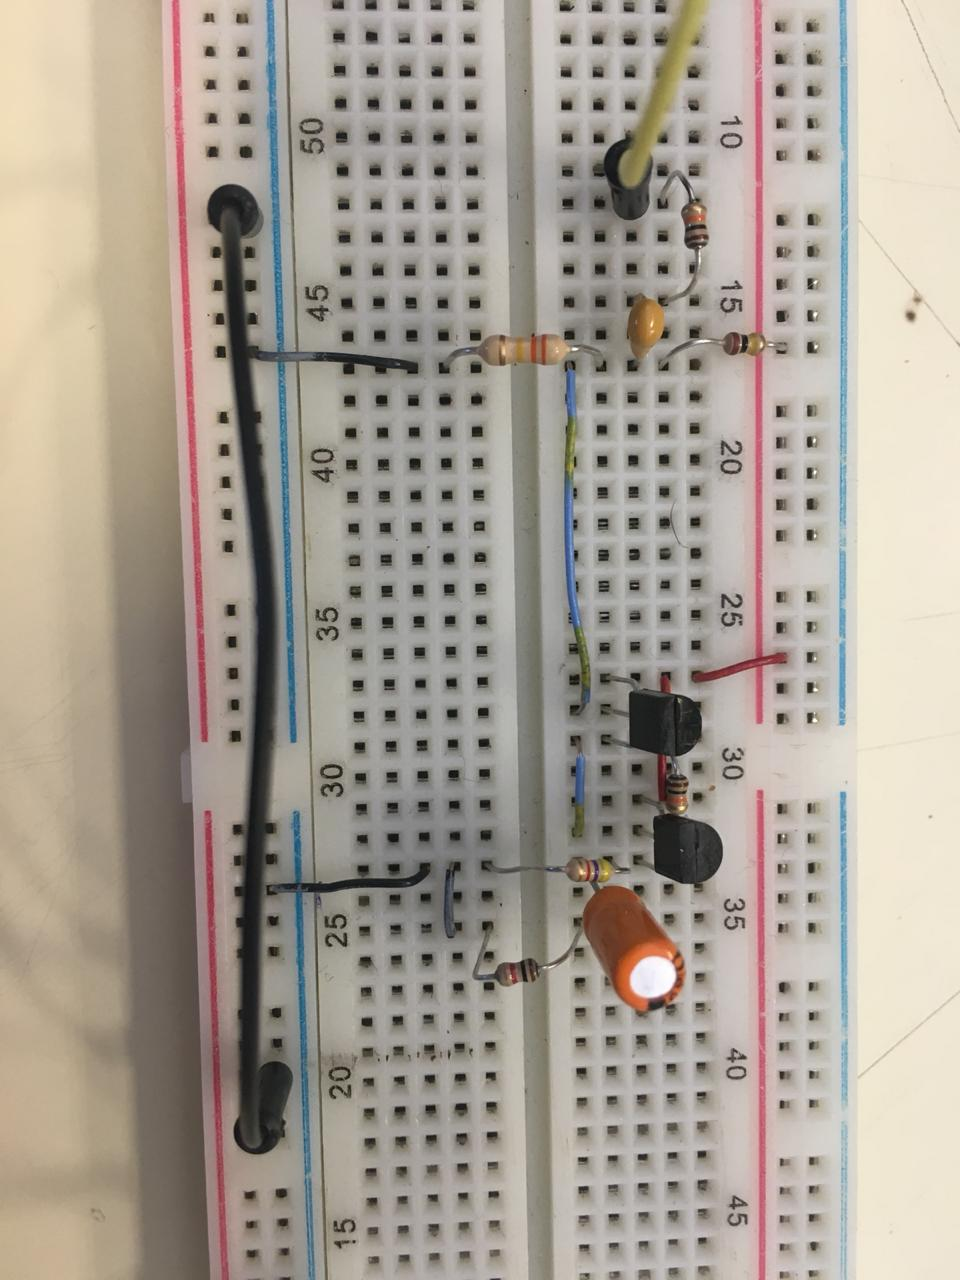
\includegraphics[scale=0.4]{./Imagenes/circuito_proto.jpeg} \\
			\caption{Circuito armado en protoboard.}
			\label{circ_proto}
		\end{figure}

\subsection{Polarización}
La comparación entre los valores de la polarización de los transistores se muestran en la Tabla\ref{tabla_polarizacion_comp}. Las diferencias en las $I_{CQ}$ se deben principalmente a las variaciones de $\beta$ con $I_{C}$, que fueron tenidas en consideración en los cálculos teóricos, pero de todas formas es distinto al real.

\todo{IAgregar columna Simulado}

	\begin{table}[h!]
	\centering
	\begin{tabular}{c c c c}%
		\bfseries &Te\'orico & Medido & Simulado \\ \hline \\
		$V_{CEQ1} (V)$ & $4,01$ &$4,00$ & \\
		$V_{CEQ2} (V)$ & $4,71$& $4,60$& \\
		$I_{CQ1} (\mu A)$ & $93,54$&$66,00$ & \\
		$I_{CQ2} (mA)$ &$2,30$ & $2,10$& \\
		$V_{BE1} (mV)$ &$700,00$ &$520,00$ & \\
		$V_{BE2} (mV)$ & $700,00$& $600,00$& \\
		\hline
	\end{tabular}
	\caption{Comparaci\'on de valores de polarizaci\'on para los casos te\'orico, medido y simulado.}
	\label{tabla_polarizacion_comp}
\end{table}

\subsection{Ganancias}
En primer lugar, se midió la ganancia de tensión del sistema. En la Figura \ref{fig_bode_avs} se muestra la constrastación de la medición, la simulación y la teoría. Como ningún cálculo teórico tiene en cuenta variaciones con la frecuencia, se toma un único valor para todas las frecuencias, y se ve que la aproximación para frecuencias medias es válida en el intervalo de frecuencias entre 400$Hz$ y 500$kHz$, donde la ganancia empieza a caer. La ganancia en la banda pasante simulada es de 0.87 veces y la medida llega hasta 0.9 veces, con lo que el cálculo teórico de 0.866 veces resulta muy cercano a la realidad.

		\begin{figure}[H]
			\centering
			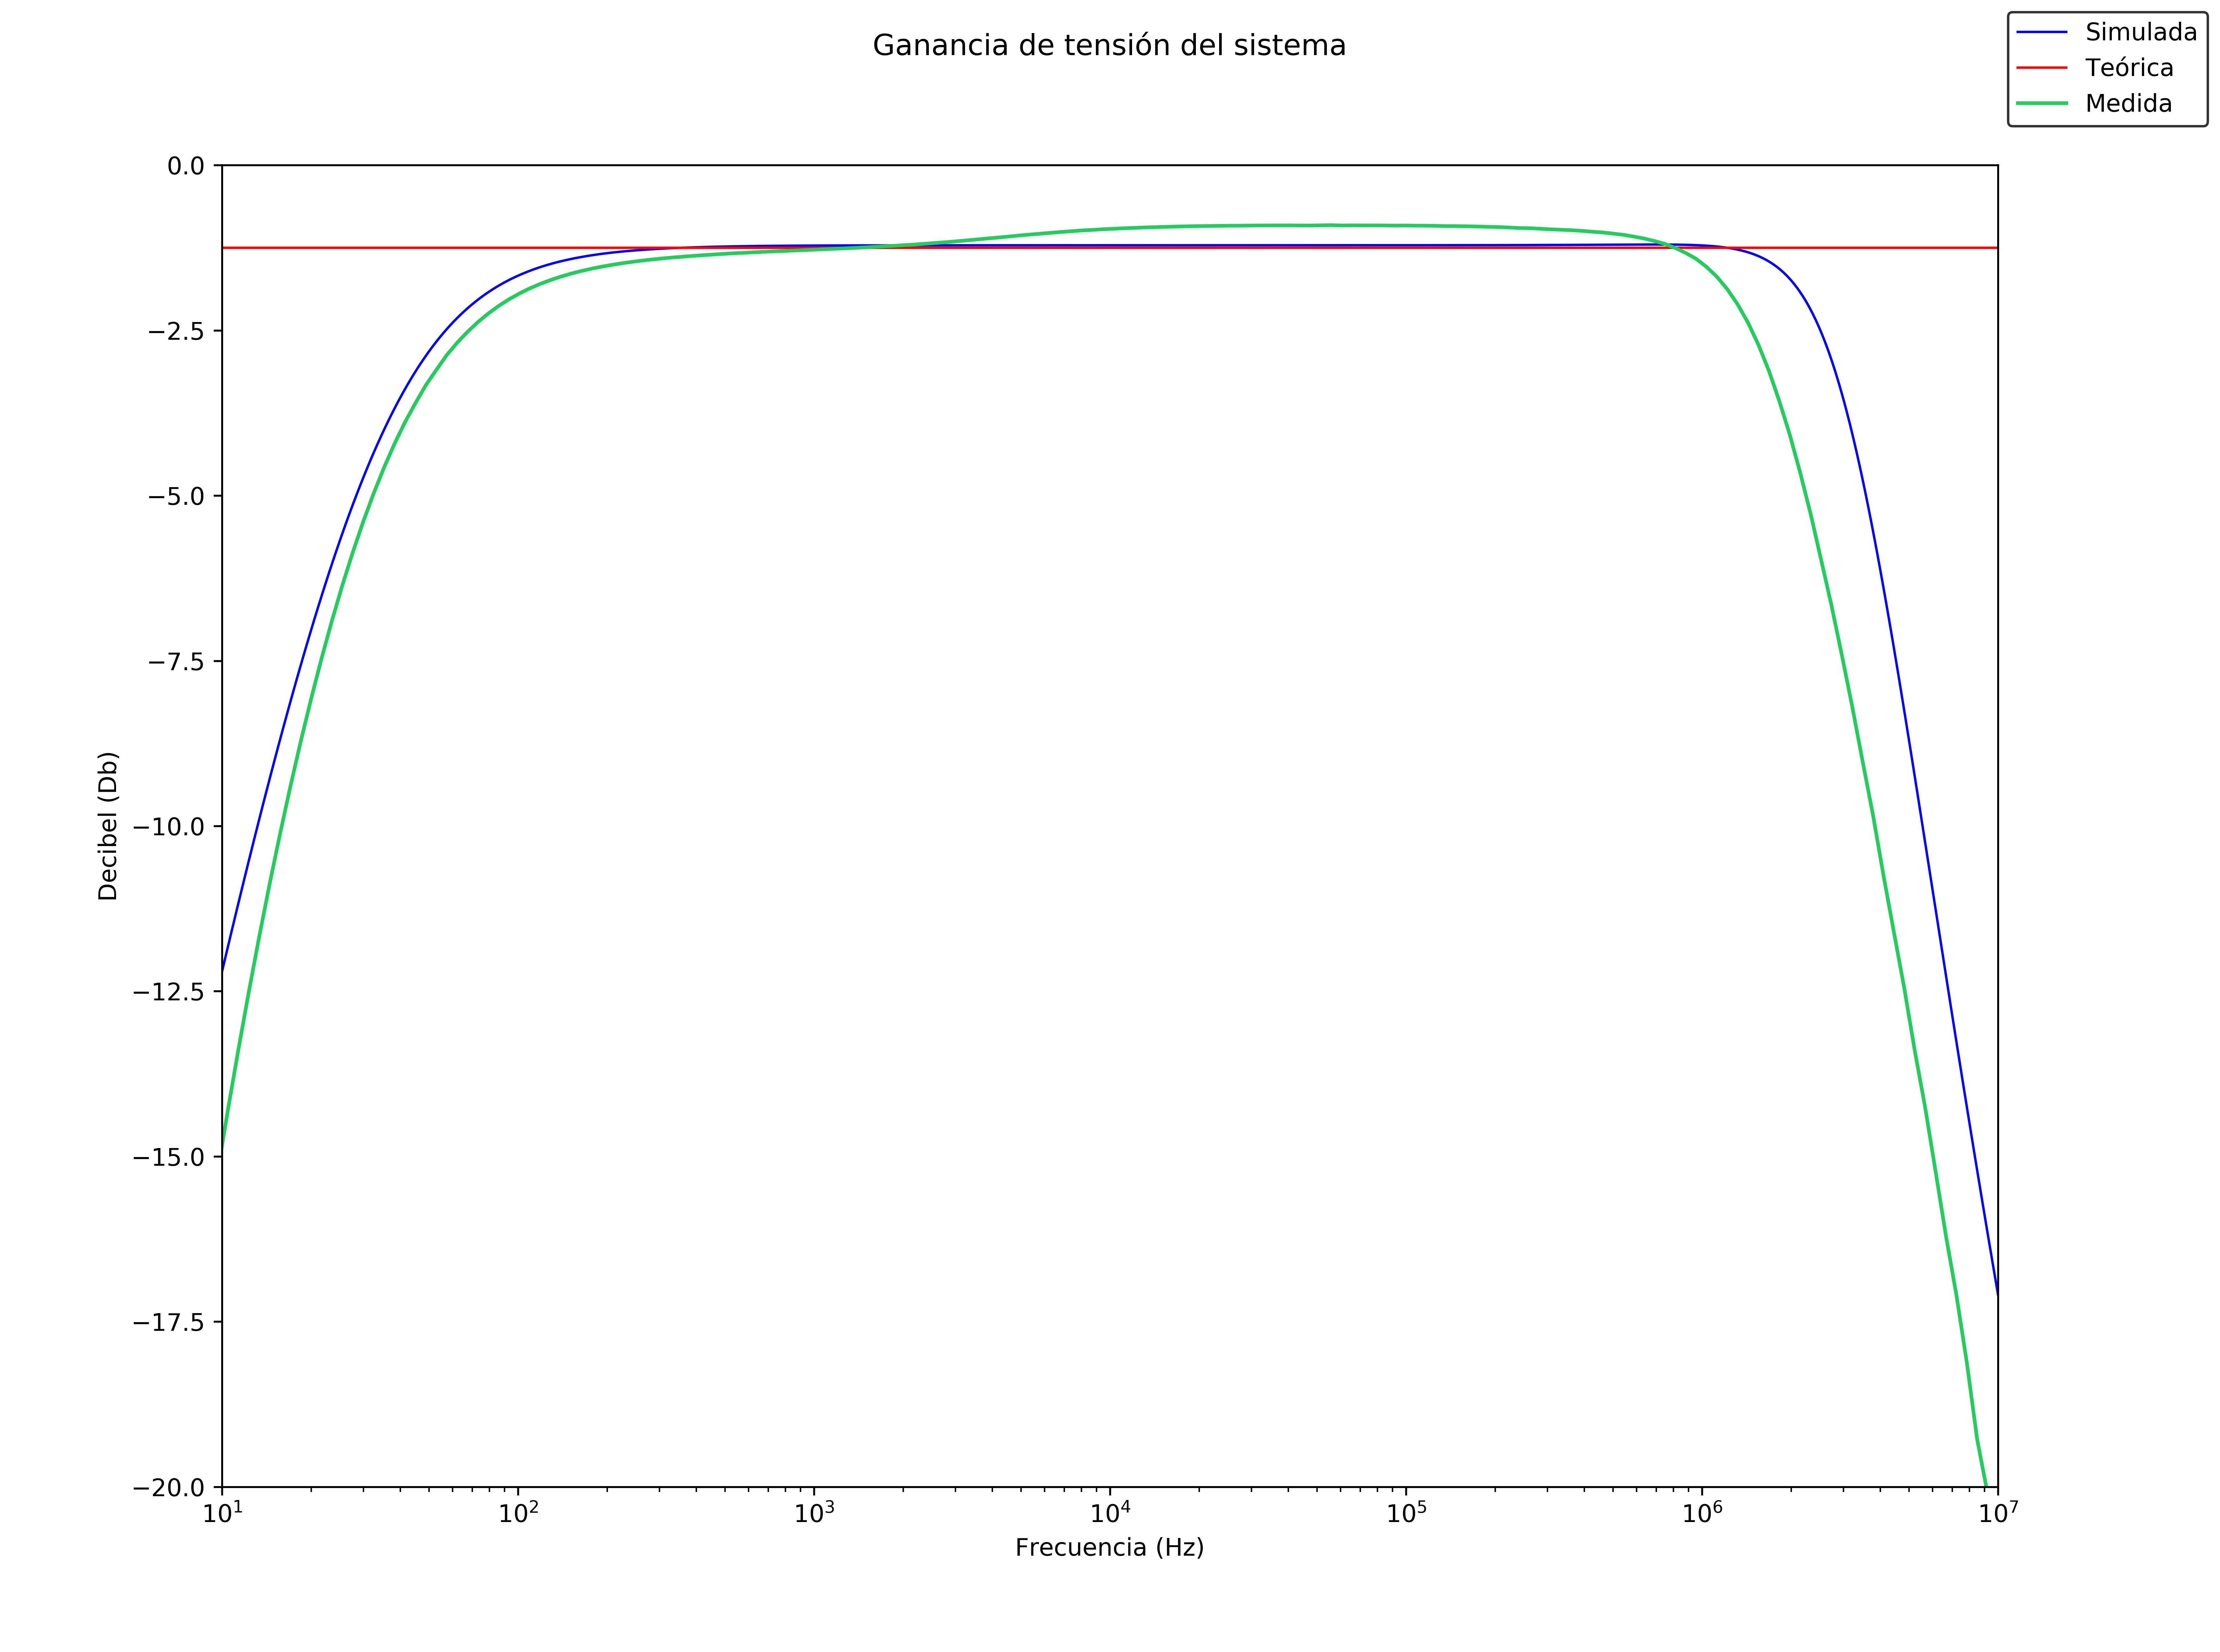
\includegraphics[scale=0.4]{./Imagenes/bode_Avs.png} \\
			\caption{Ganancia de tensión del sistema teórica, simulada y medida}
			\label{fig_bode_avs}
		\end{figure}

Luego se midió la ganancia de corriente del sistema. En la Figura \ref{fig_bode_ais} se puede observar la comparación entre teoría, simulación y práctica. En éste caso, es menor el intervalo de frecuencias en las que es válida la estimación teórica, y se presenta una diferencia entre simulación y medición en el punto en el que empieza a caer la ganancia. Éste efecto puede ser atribuible a las capacidades introducidas por el protobard. La ganancia en la banda pasante simulada y medida es de 37,5dB, es decir, 75 veces, mientras que la teórica es de 74 veces, con lo que el modelo nuevamente se verifica. 

\todo{Insertar valores más específicos de simulación y medición}

		\begin{figure}[H]
			\centering
			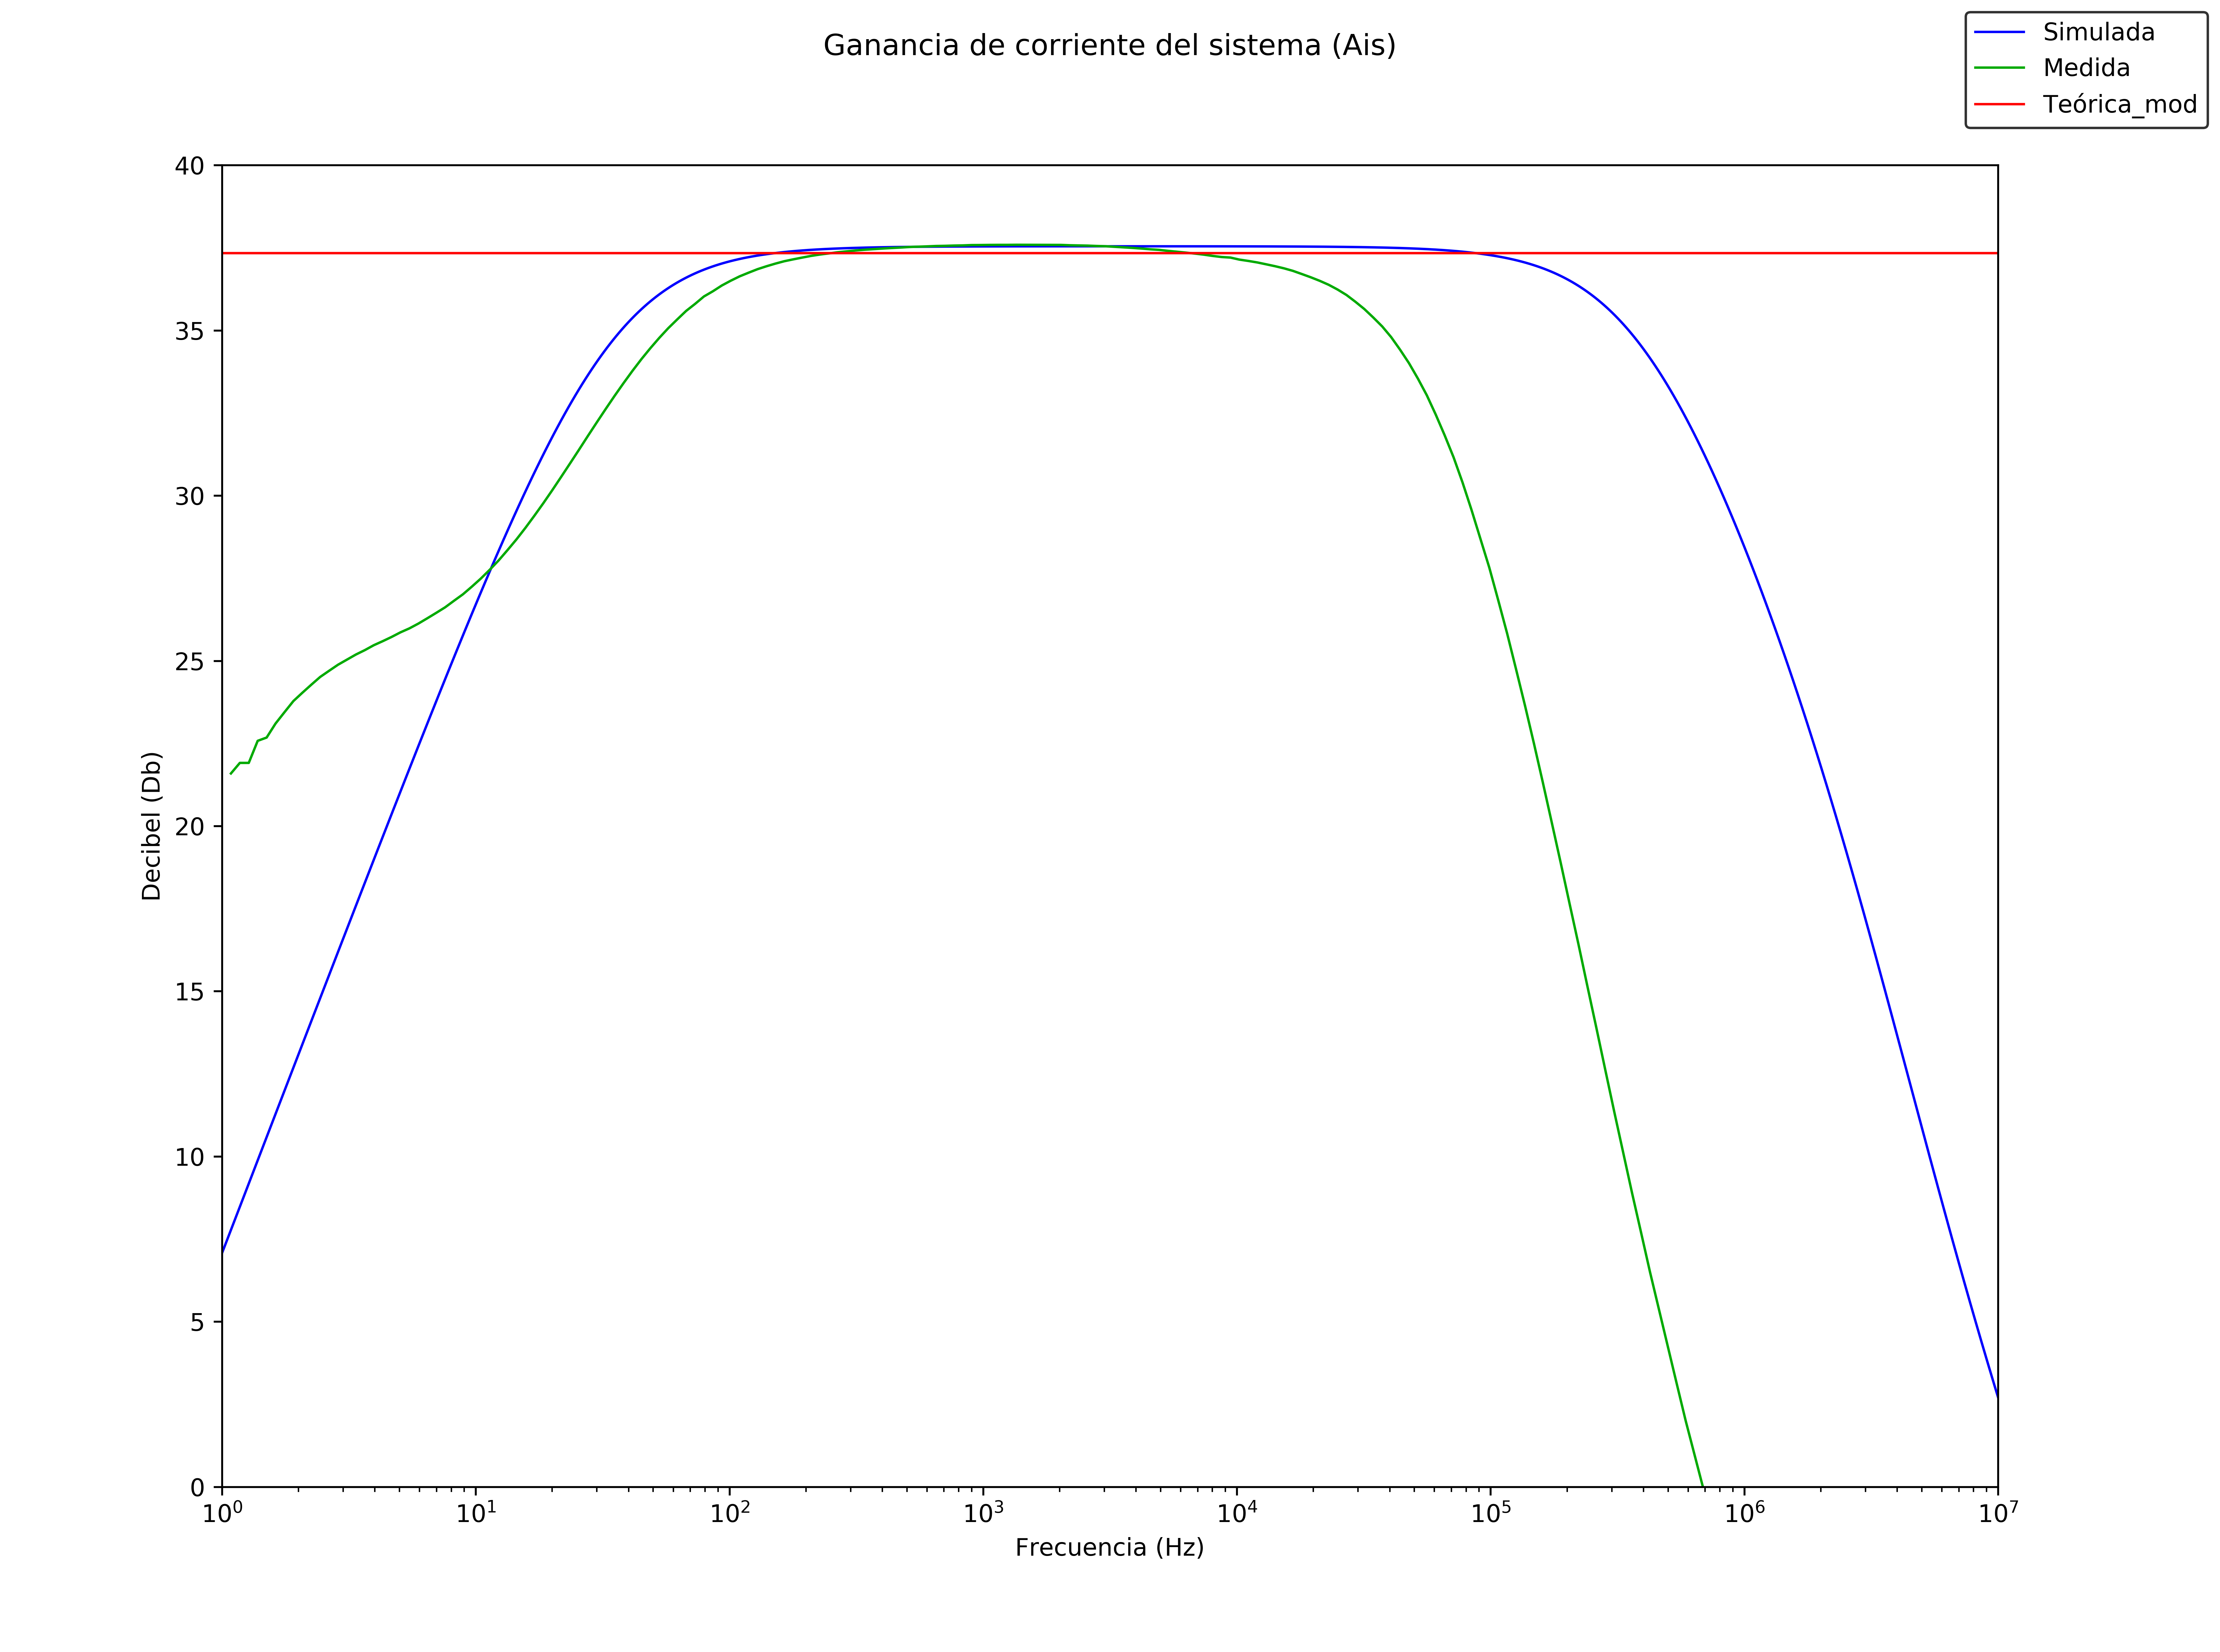
\includegraphics[scale=0.3]{./Imagenes/bode_Ais.png} \\
			\caption{Ganancia de corriente del sistema teórica, simulada y medida}
			\label{fig_bode_ais}
		\end{figure}

\subsection{Impedancias}
Con respecto a la impedancia de entrada, se muestra la contrastación entre teoría, simulación y medición en la Figura \ref{fig_bode_zin}, donde se puede apreciar que para frecuencias inferiores a 10$kHz$ las tres curvas son cercanas, siendo la impedancia de entrada medida a 200Hz $76,2k\Omega$, mientras que la simulada a la misma frecuencia es de $86,676k\Omega$ y la teórica es de $85k\Omega$. Nuevamente se observa que la medición no se corresponde con la medición a partir de 10$kHz$.

		\begin{figure}[H]
			\centering
			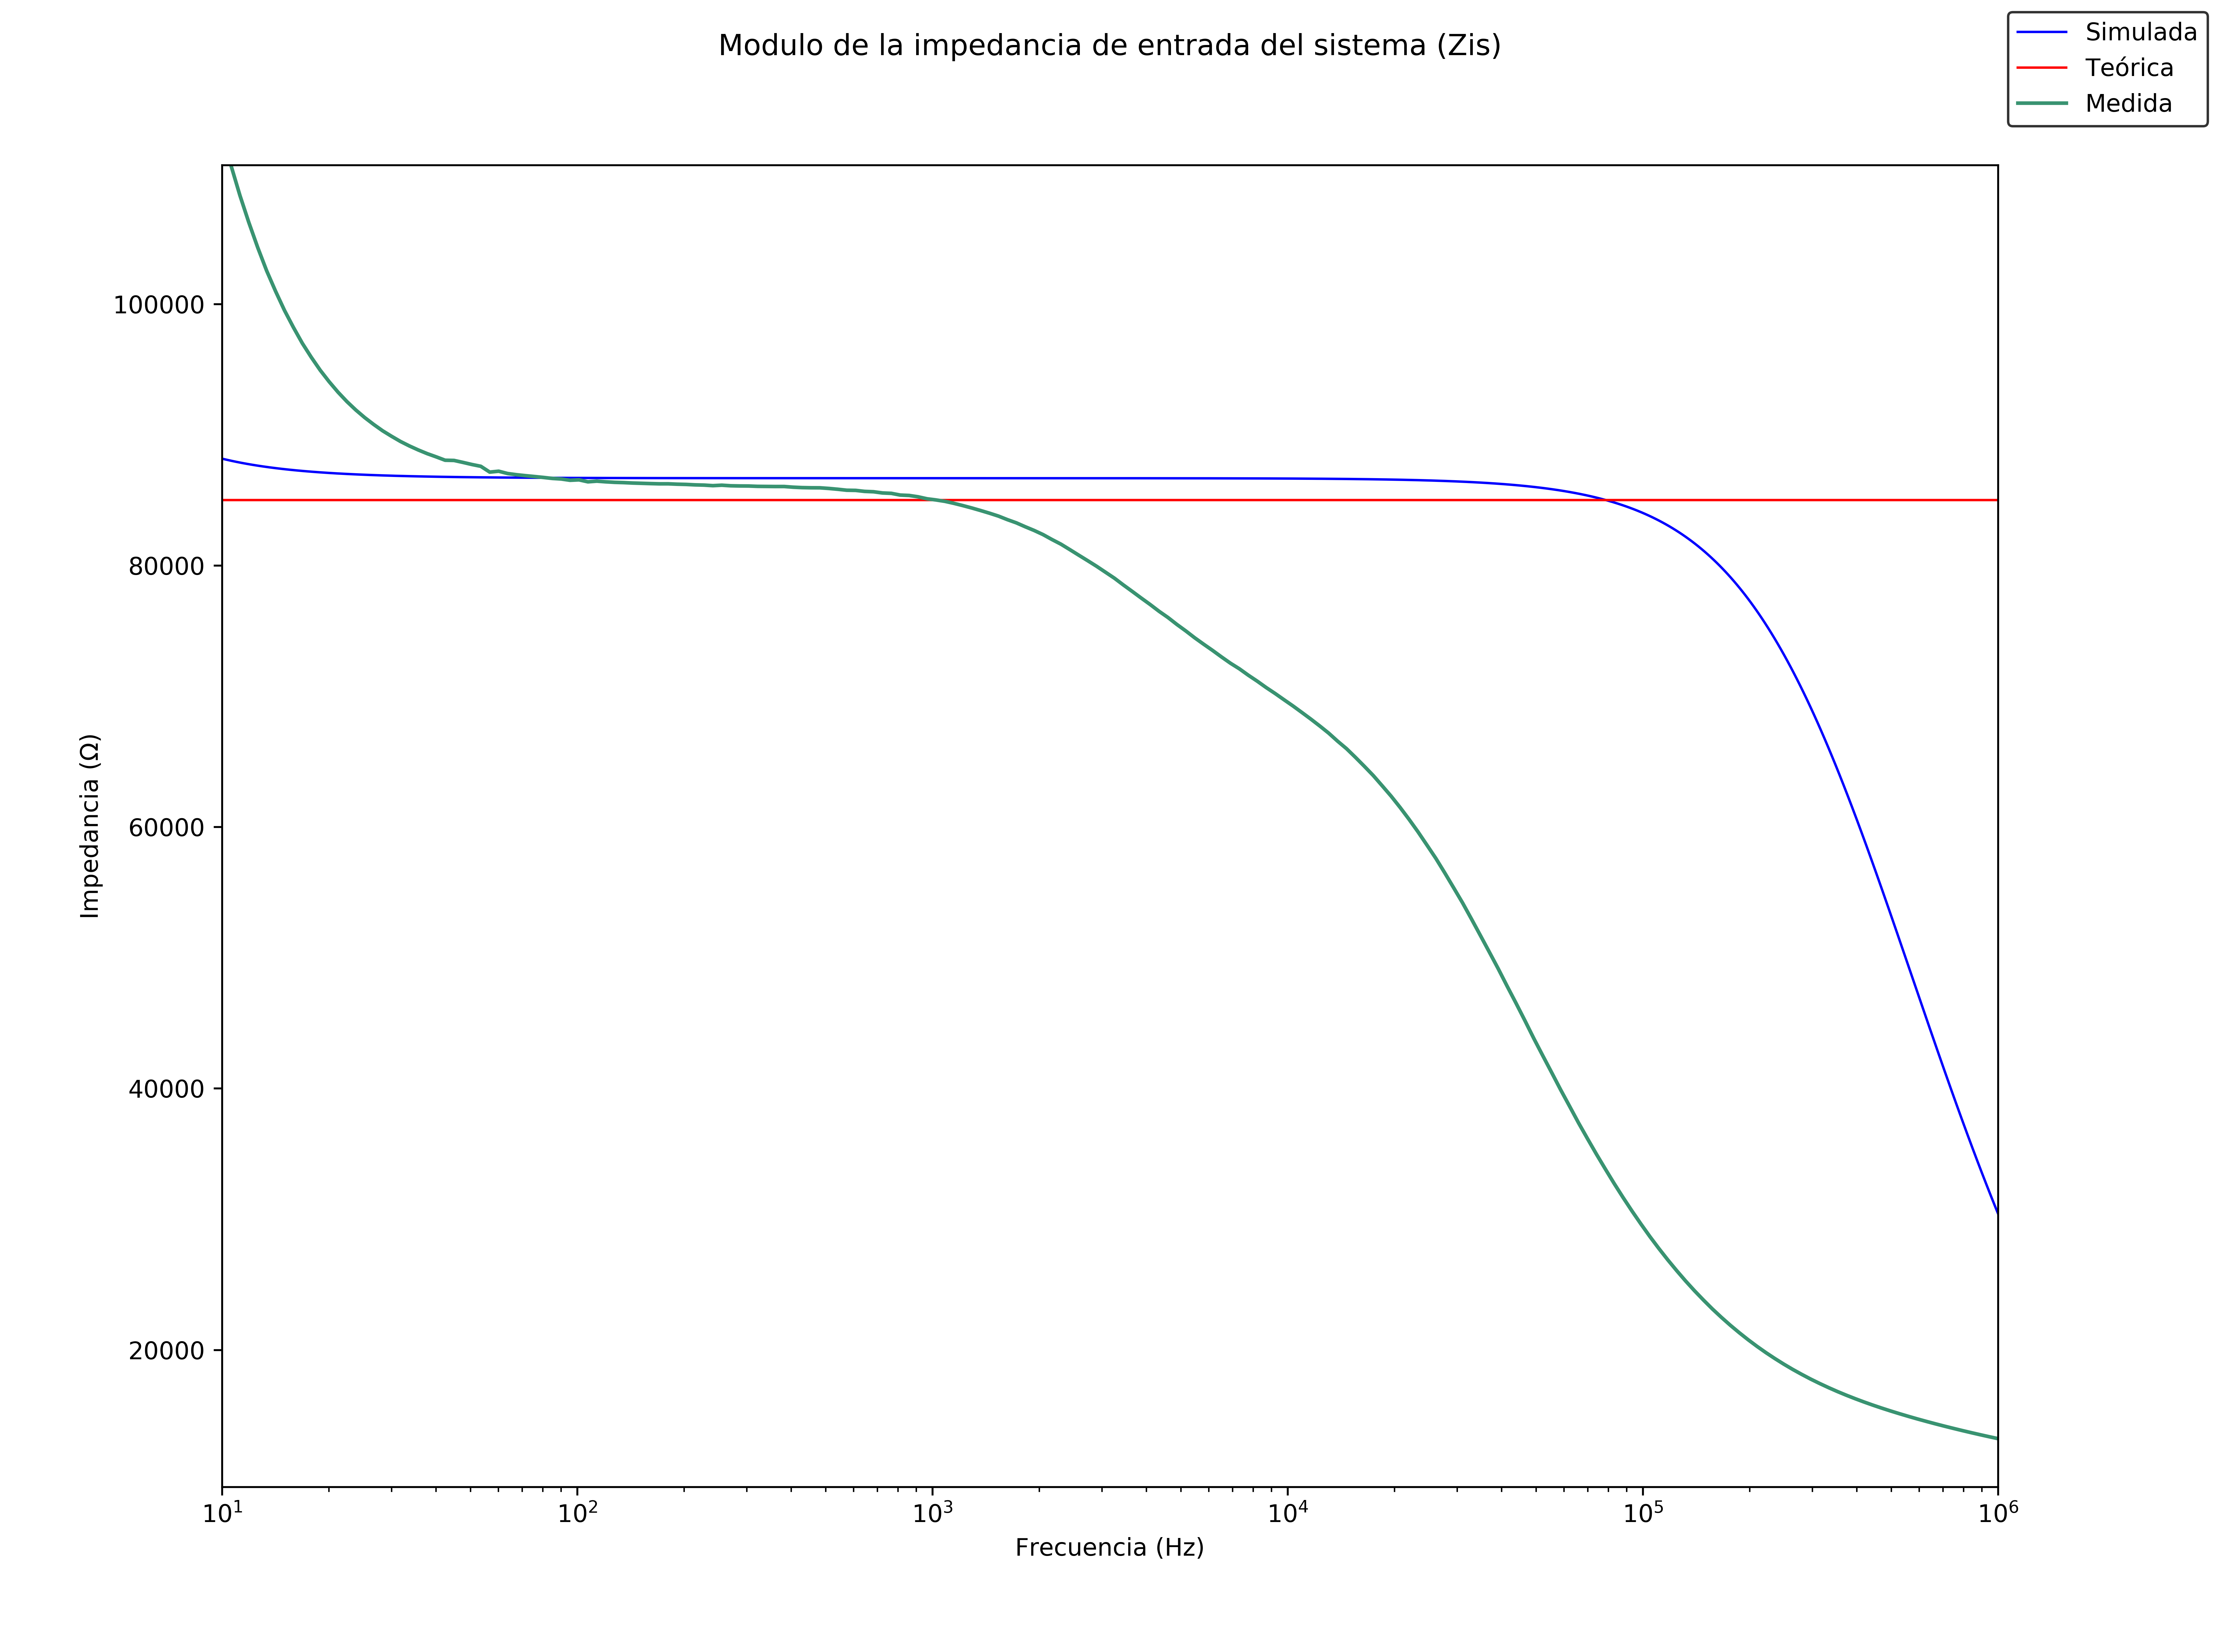
\includegraphics[scale=0.4]{./Imagenes/Modulo_zin.png} \\
			\caption{Impedancia de entrada del sistema teórica, simulada y medida.}
			\label{fig_bode_zin}
		\end{figure}

Para la impedancia de salida se muestra la contrastación entre teoría, simulación y práctica en la Figura \ref{fig_bode_zout}. Se observa que el sistema presenta una baja impedancia de salida, lo cual era esperado por tratarse de un colector común. 

\todo{Insertar valores}

		\begin{figure}[H]
			\centering
			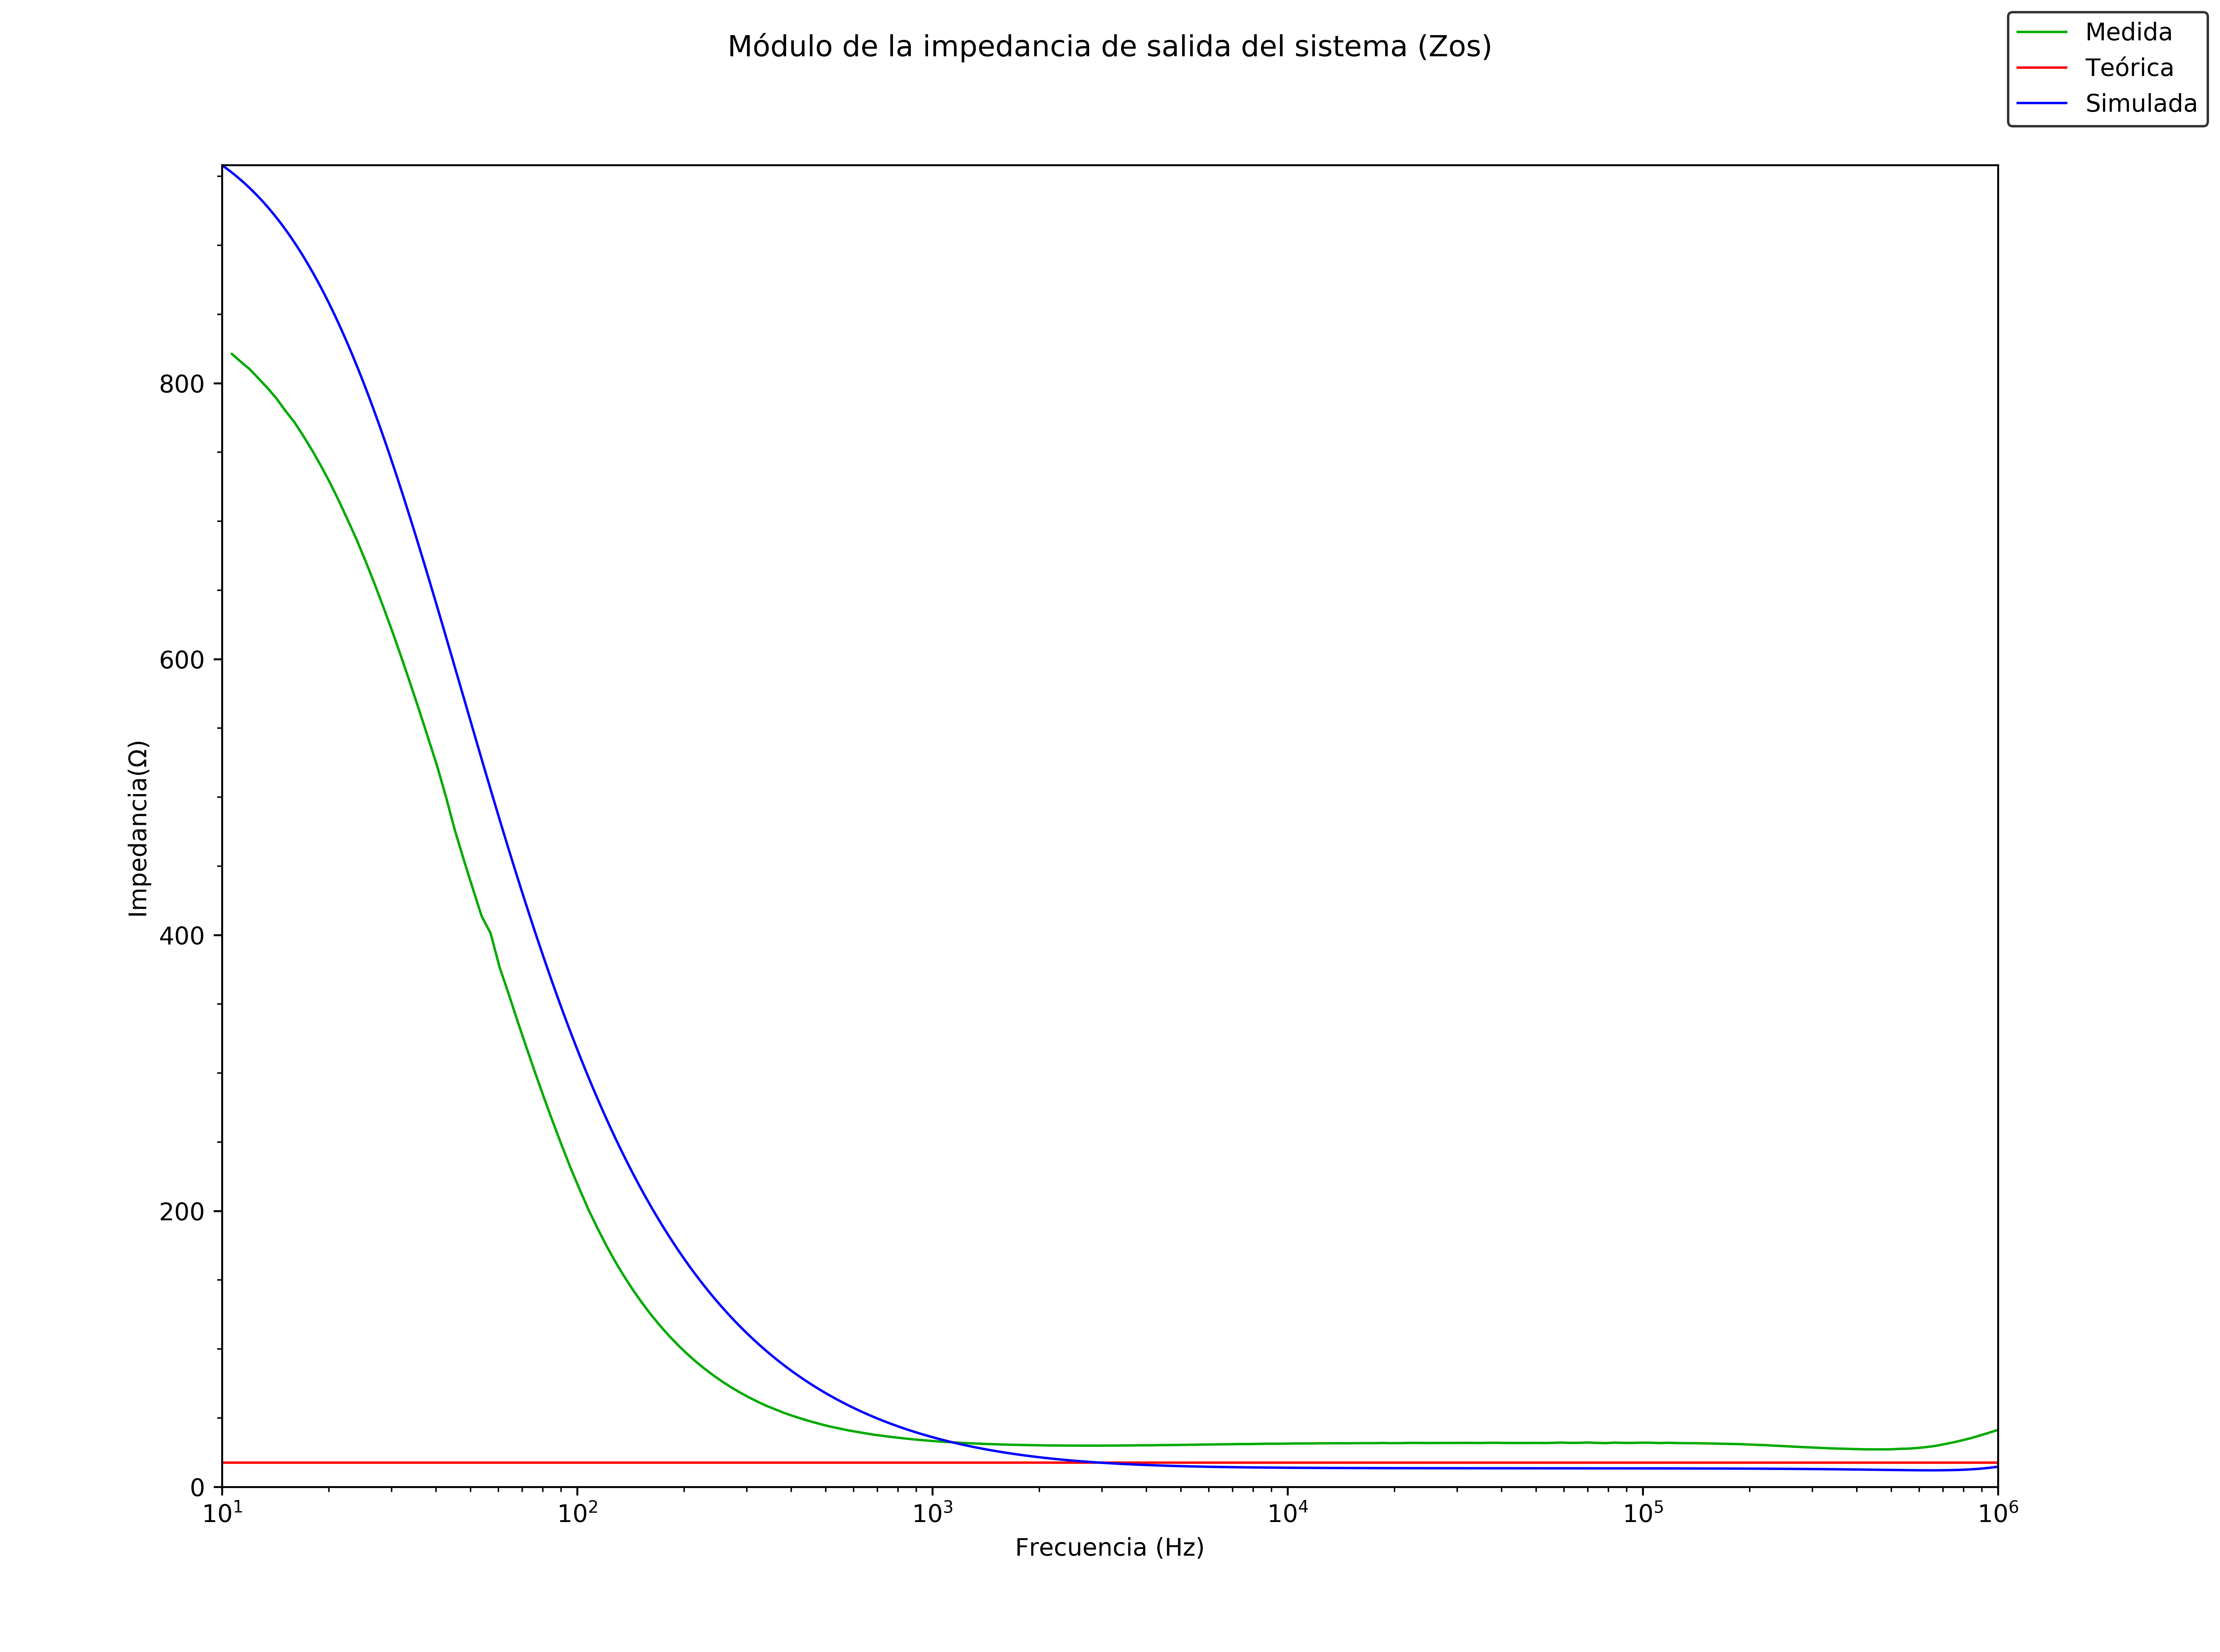
\includegraphics[scale=0.4]{./Imagenes/Modulo_zos.png} \\
			\caption{Impedancia de salida del sistema teórica, simulada y medida.}
			\label{fig_bode_zout}
		\end{figure}
 
\subsection{Resumen}

En la siguiente tabla se muestran los valores teóricos, simulados y medidos de las ganancias e impedancias para frecuencias medias. Se tomaron los valores para %___ kHz


\todo{Insertar tabla con los valores para frecuencias medias que den lindo, buscar en txt de simulaciones y csv de mediciones los que no estén puestos más arriba}
\newpage
\section{Conclusi\'on}
\end{document}